\section{Data analysis}
As no data was surveyed by the authors, there will be no chapter on the experimental procedure. Instead, the focus will be on the analysis of the data, for most of which the framework ROOT was used. Data was provided from two sources:
\begin{enumerate}
	\item Monte Carlo simulations, separated by decay reaction.
	\item Actual data from the OPAL detector at the LEP collider.
\end{enumerate}


\subsection{Selection of cuts}
In a first step, the data from the Monte Carlo simulations is plotted over adequate range in the following parameters:
\begin{itemize}
	\item{\makebox[3cm][l]{\textbf{NCHARGED:}}The number of tracks visible in the drift chamber}
	\item{\makebox[3cm][l]{\textbf{PCHARGED:}}Energy of particles that left a track in the drift chamber}
	\item{\makebox[3cm][l]{\textbf{E\_ECAL:}}Energy deposited in the electromagnetic calorimeter}
	\item{\makebox[3cm][l]{\textbf{E\_HCAL:}}Energy deposited in the hadronic calorimeter}
	\item{\makebox[3cm][l]{\textbf{COS\_THET:}}Angle $\theta$ between created the positive lepton and the \\\makebox[3cm][l]{}incident positron beam}
	\item{\makebox[3cm][l]{\textbf{COS\_THRU:}}Angle between the thrust axis for hadronic events and the \\\makebox[3cm][l]{}incident positron beam}
\end{itemize}
These plots include the simulation events from decays to electrons, myons, tauons as well as quarks in similar amounts. These ratios are not a representation of the actual ratios as they would be expected in the real data, as the decay width of quarks is much greater than that of the three types of leptons. \\
To further improve comparability of the different data sets, all histograms were normed to an integral of 1. The resulting plots are shown in figures \ref{fig:Ncharged} to \ref{fig:cos_thru}. Using these graphs, as well as the knowledge of the type of event, cuts are established which will later be used to separate the actual data, where there is no initial knowledge of the type of event.\\
Thus, for every type of educts, a cut is to be made with maximum possible efficiency in detecting the respective kind of event, as well as maximum purity, meaning that other events are falsely allotted as rarely as possible.

\newpage
\begin{figure}[H]
\centering
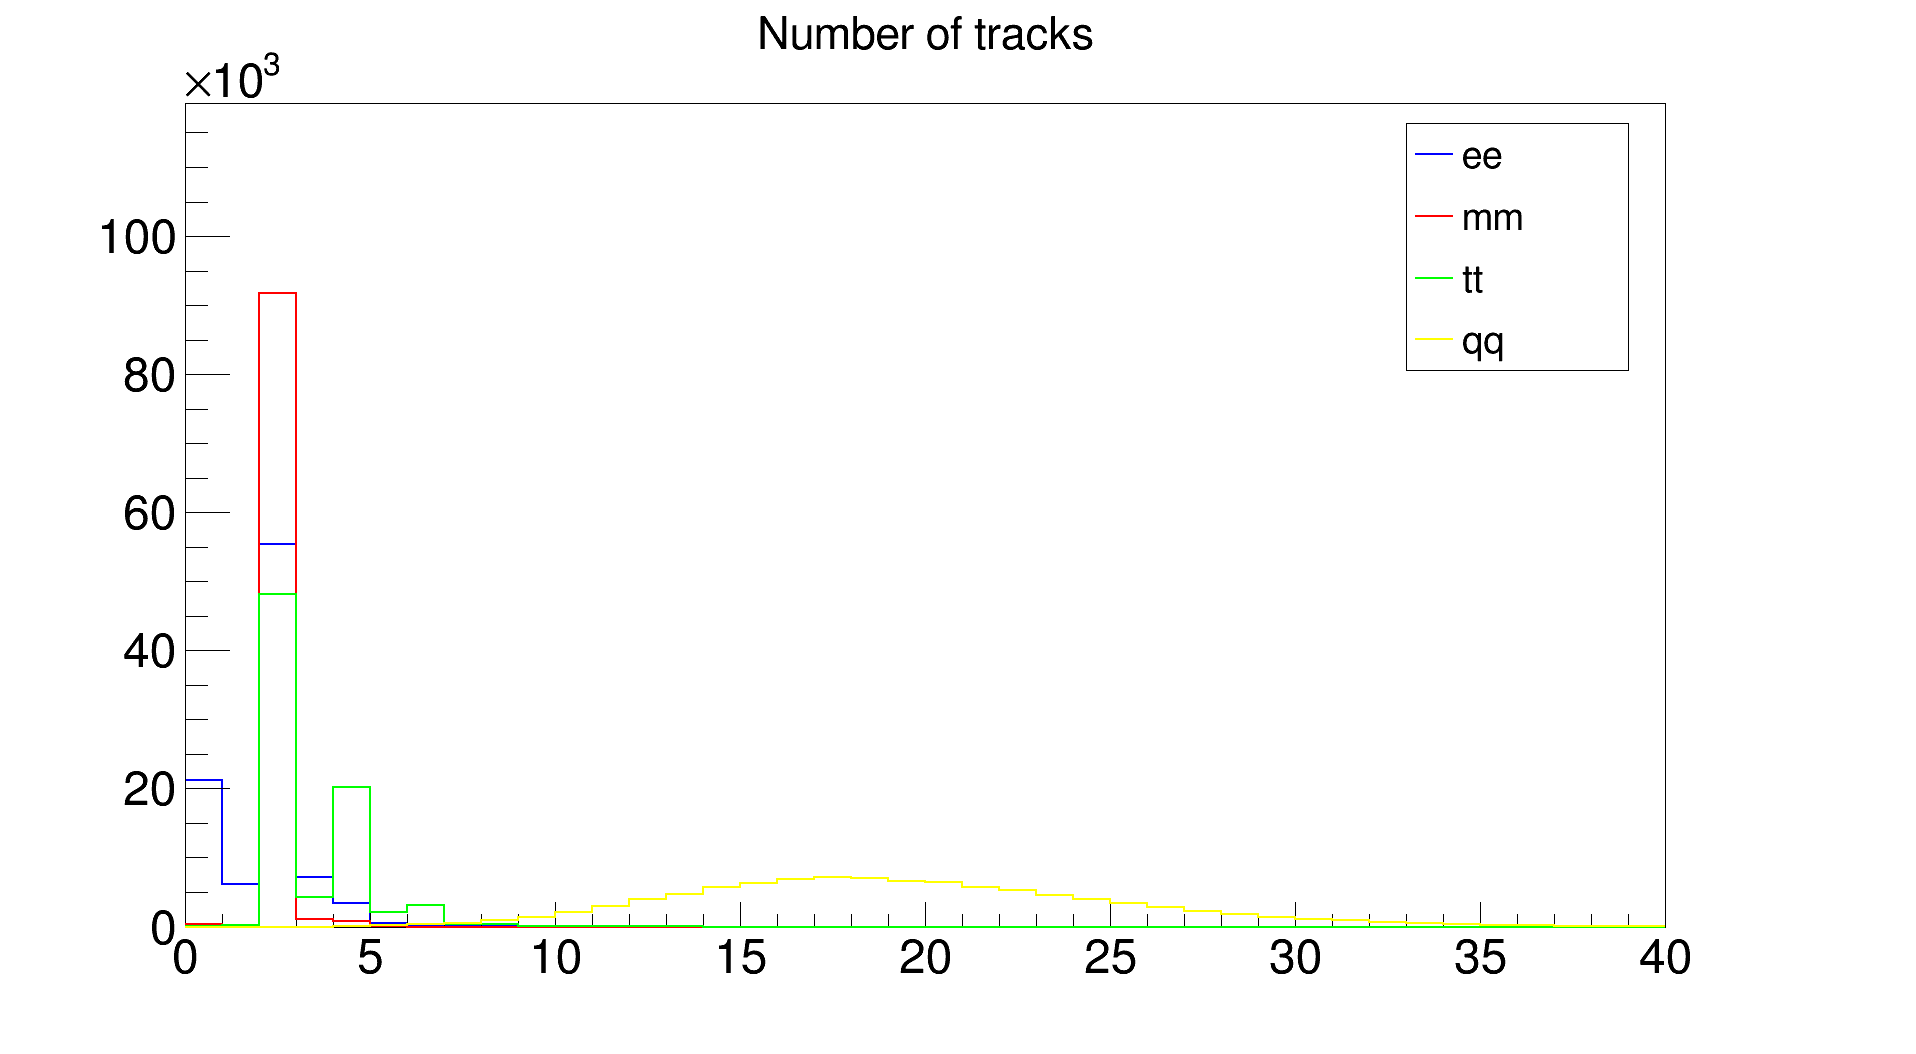
\includegraphics[width=1\linewidth]{../results/MC_results/nocut/Ncharged}
\caption[Ncharged in simulation data]{The number of charged tracks in the simulation data for the various decay events (color-coded). Almost all muon events leave two tracks. The peak is cut off to increase visibility of the other data.}
\label{fig:Ncharged}
\end{figure}

\subsubsection{Cuts in Ncharged}
Above figure suggests a good way to separate the data sets. In particular, all three lepton generations hardly ever leave more than 6 tracks, with muons hardly having anything but two tracks in the drift chamber. This suggests the following cuts:

\begin{itemize}
	\item{\makebox[2.5cm][l]{\textbf{Lepton cuts:}} Ncharged $<7$}
	\item{\makebox[2.5cm][l]{\textbf{Quark cut:}} Ncharged $\ge8$}
	\item{\makebox[2.5cm][l]{\textbf{Muon cut:}} Ncharged $=2$}
\end{itemize}



\newpage
\begin{figure}[H]
\centering
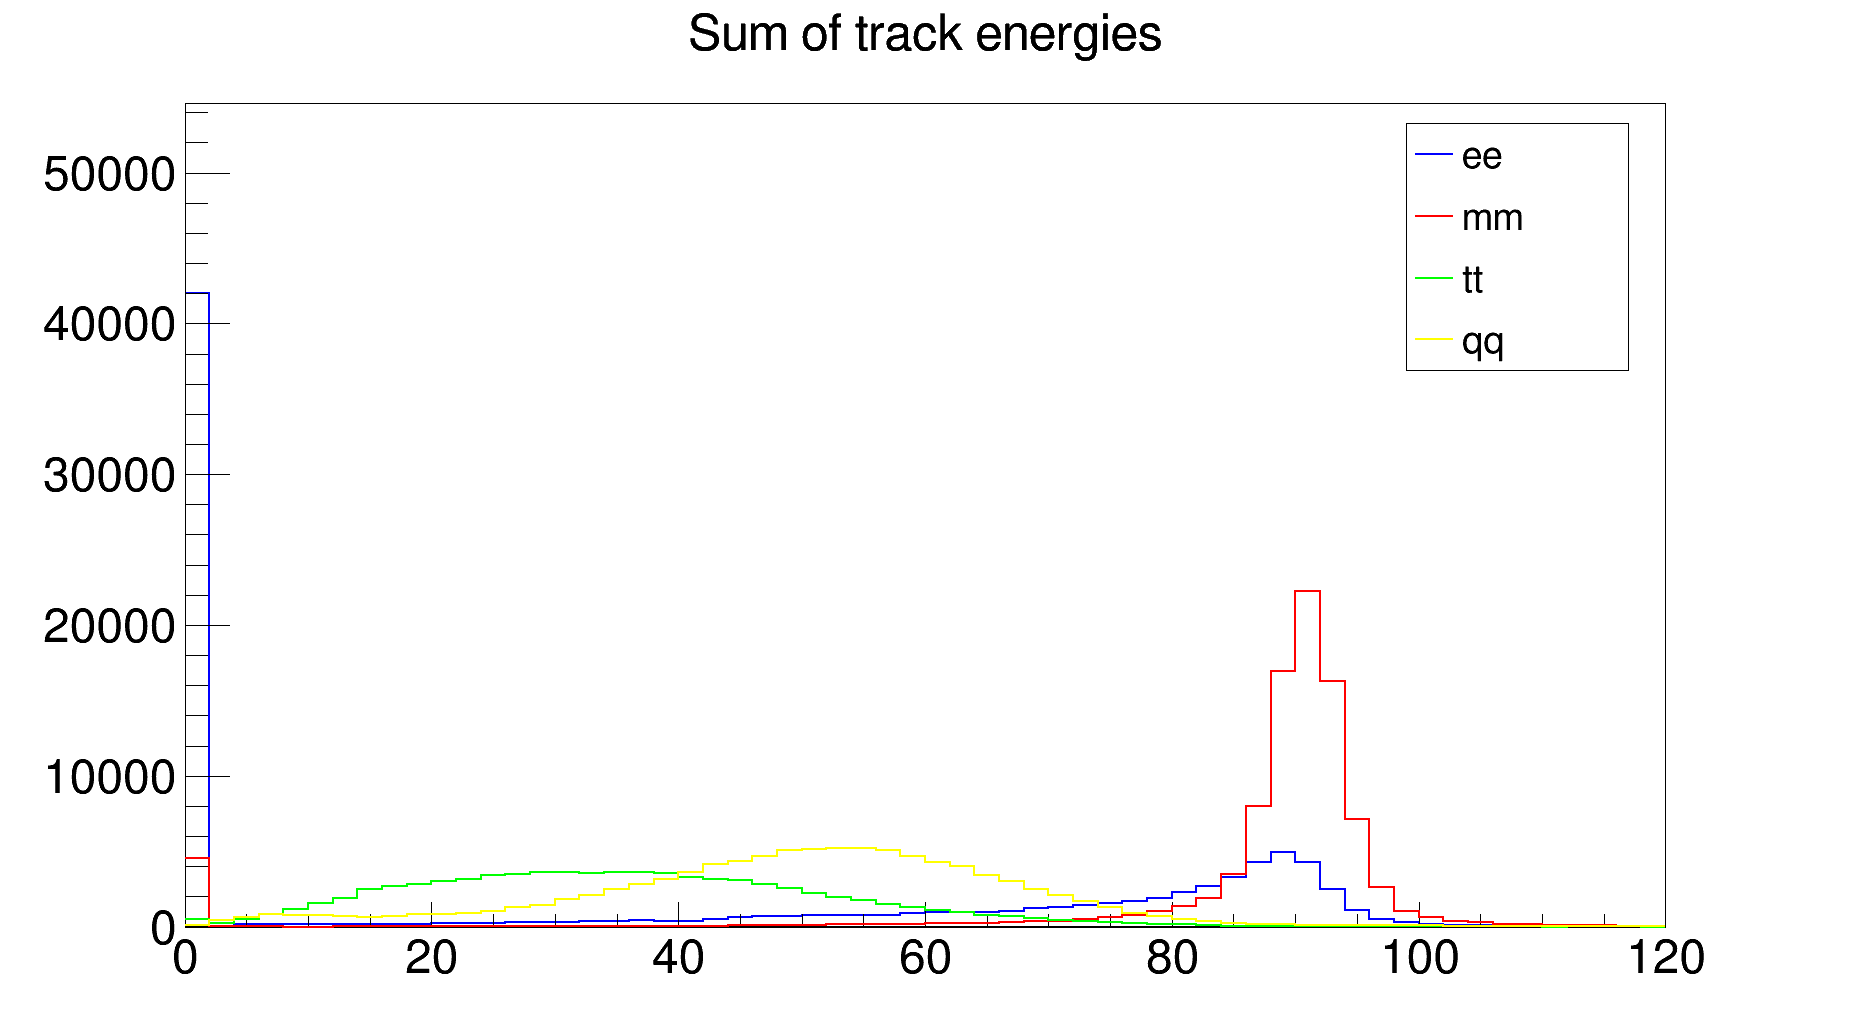
\includegraphics[width=1\linewidth]{../results/MC_results/nocut/Pcharged}
\caption[Pcharged in simulation data]{This figure shows the sum of track energies in the simulation data. }
\label{fig:Pcharged}
\end{figure}

\subsubsection{Cuts in Pcharged}
The separation of the data sets is less obvious in the Pcharged channel. Most datasets overlap, preventing the very clean cuts as they were in the Ncharged channel. However, since we have conveniently already cut against quarks in the Ncharged channel, we can ignore said dataset and separate tauons and muons as follows:
\begin{itemize}
	\item{\makebox[2.5cm][l]{\textbf{Muon cut:}} Pcharged $\le60$ GeV}
	\item{\makebox[2.5cm][l]{\textbf{Tauon cut}} Pcharged $>71$ GeV}
\end{itemize}

\newpage
\begin{figure}[H]
\centering
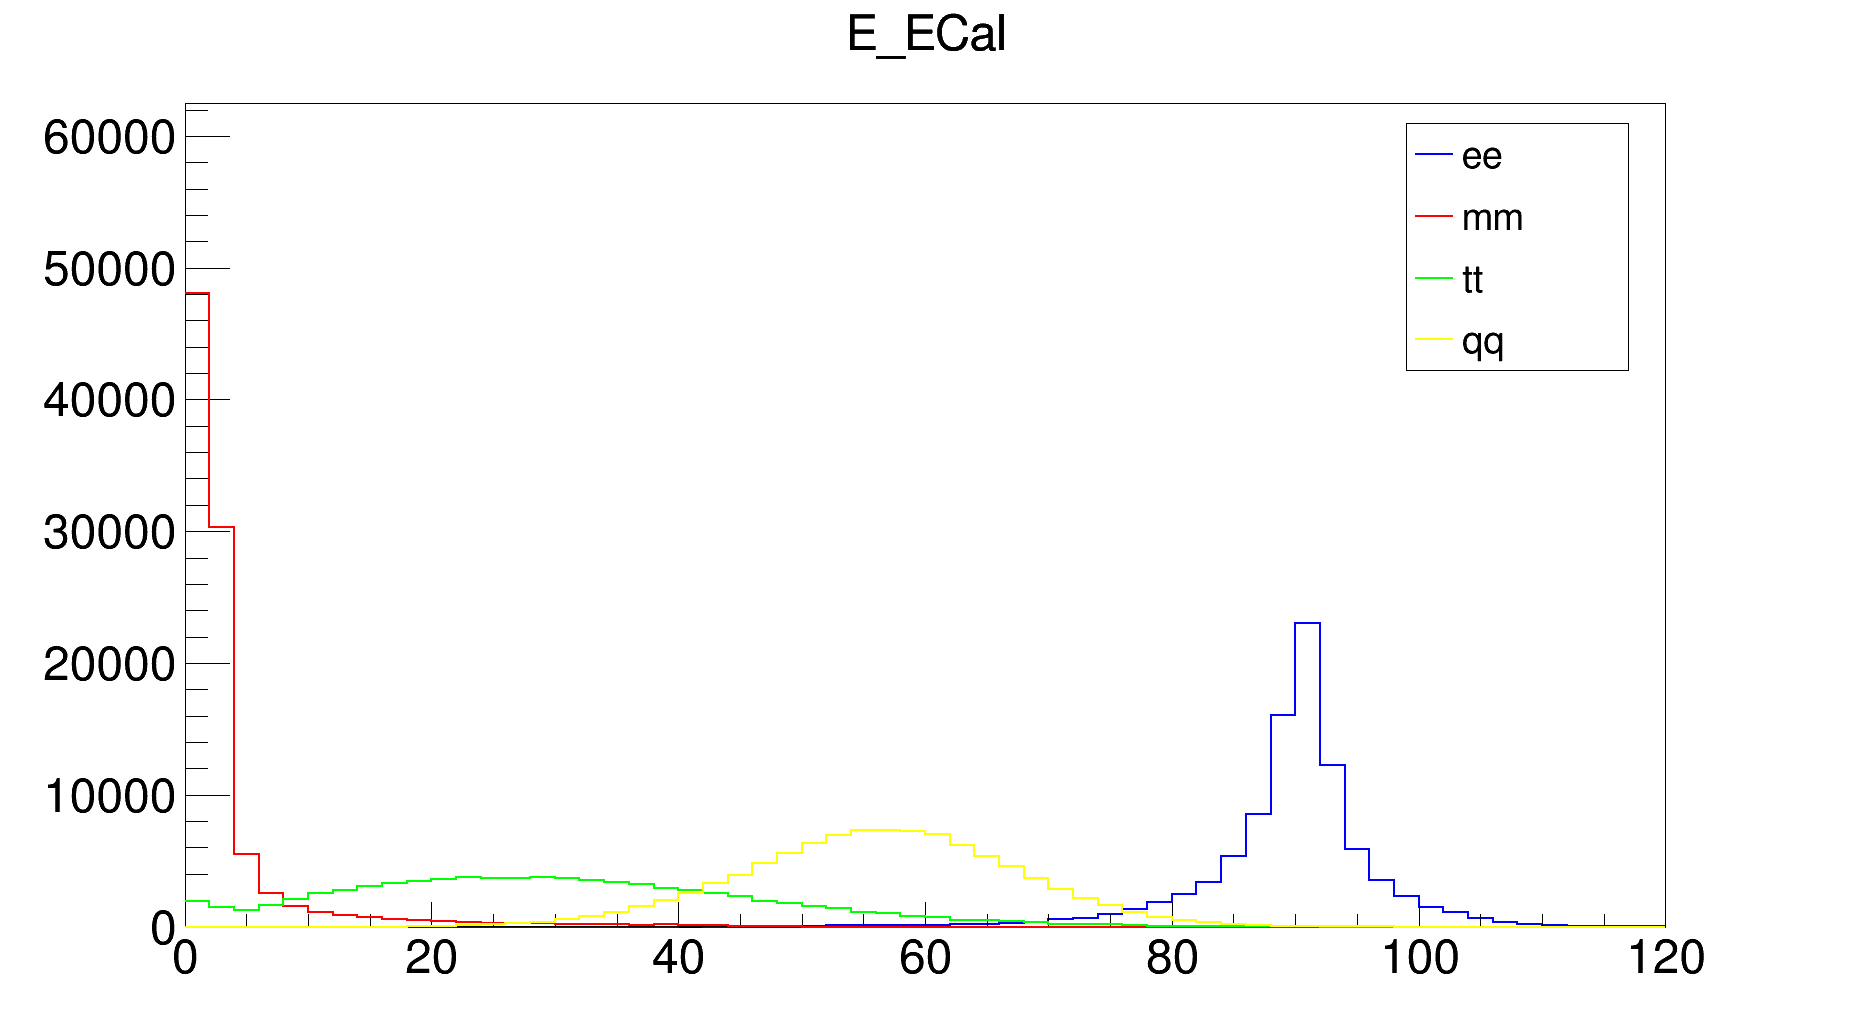
\includegraphics[width=1\linewidth]{../results/MC_results/nocut/E_Ecal}
\caption[E\_Ecal in simulations]{The energies deposited in the electronic calorimeter show clear differences for the four decay types and allow for effective cuts.}
\label{fig:E_Ecal}
\end{figure}

\subsubsection{Cuts in E\_Ecal}
As has been the case for the cuts in Pcharged, we can ignore the quark data. Instead, cuts for all leptons are applied in order to separate the three kinds:

\begin{itemize}
	\item{\makebox[2.5cm][l]{\textbf{Electron cut}} E\_Ecal $\ge70$ GeV}
	\item{\makebox[2.5cm][l]{\textbf{Muon cut:}} E\_Ecal $<50$ GeV}
	\item{\makebox[2.5cm][l]{\textbf{Tauon cut:}} E\_Ecal $<60$ GeV}
\end{itemize}

\newpage
\begin{figure}[H]
\centering
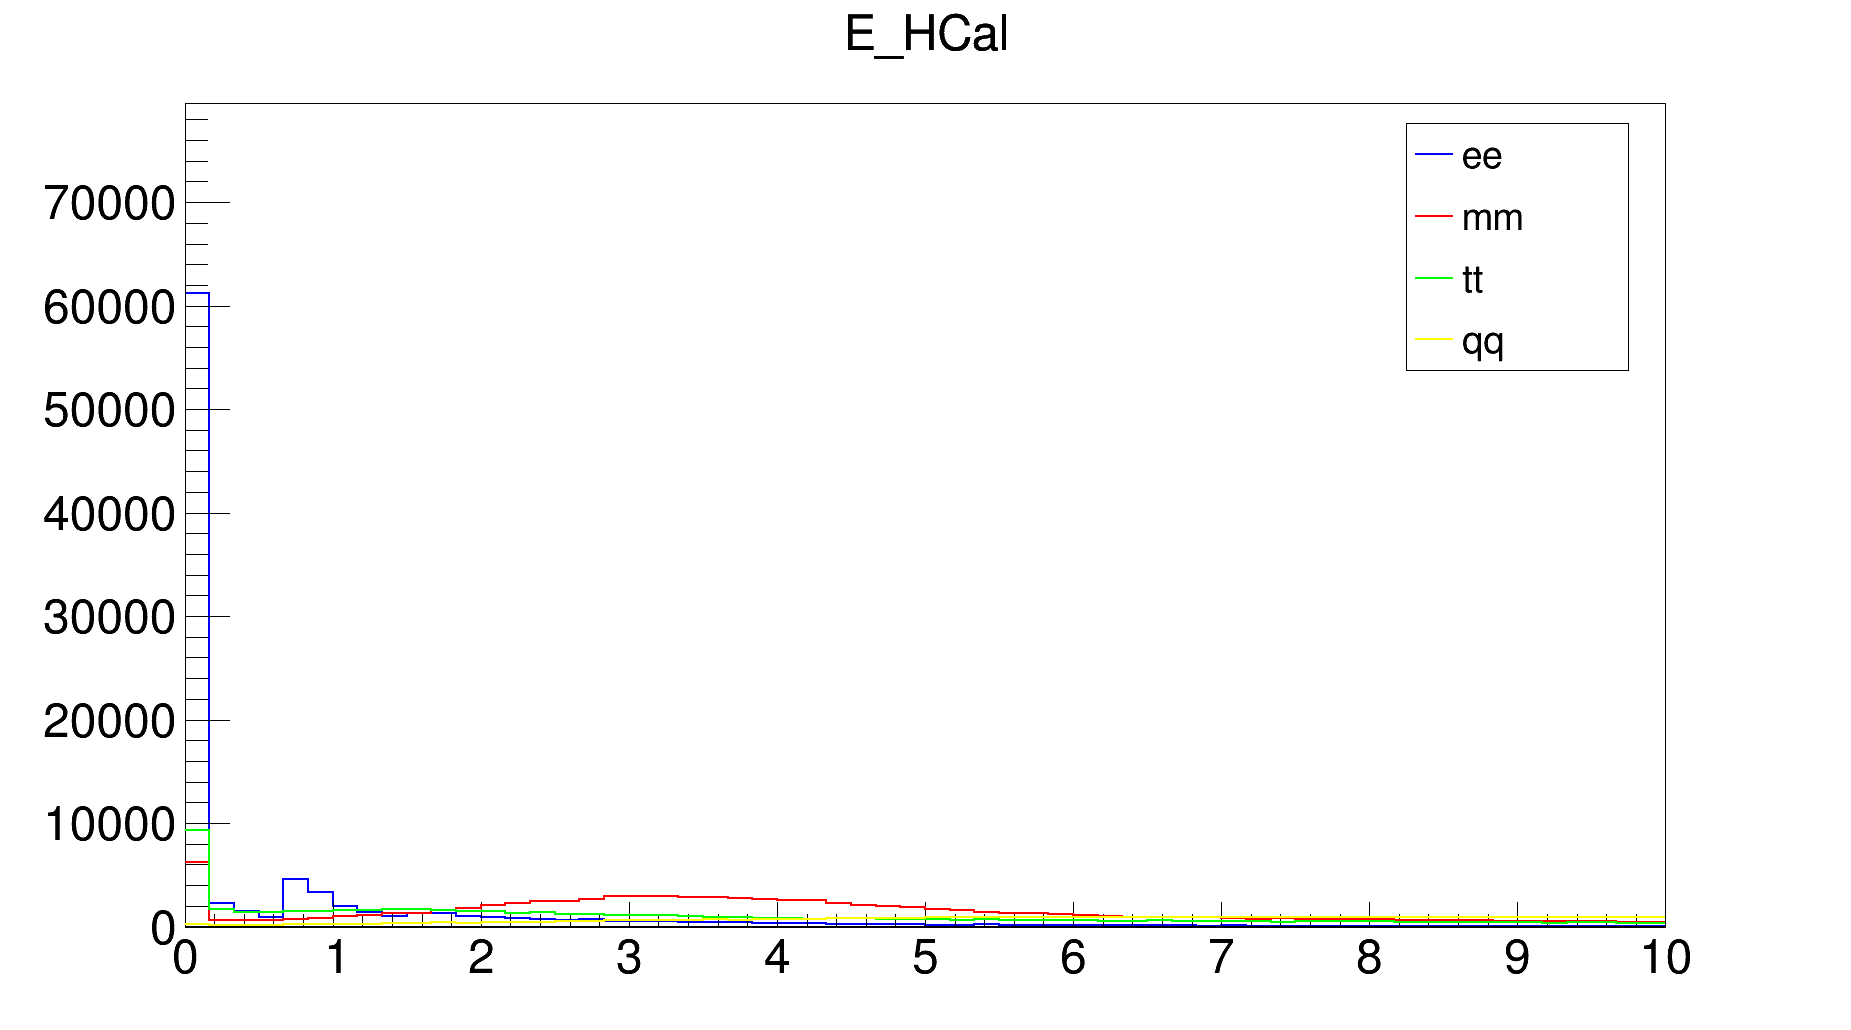
\includegraphics[width=1\linewidth]{../results/MC_results/nocut/E_Hcal}
\caption[E\_Hcal in simulation data]{The plot shows the energies deposited in the hadronic calorimeter. The distribution of the decay types overlap significantly.}
\label{fig:E_Hcal}
\end{figure}

\subsubsection{Cuts in E\_Hcal}
In the data from the hadronic calorimeter, the overlap between all four kinds of decay events does not allow for any kind of meaningful cuts.

\newpage
\begin{figure}[H]
\centering
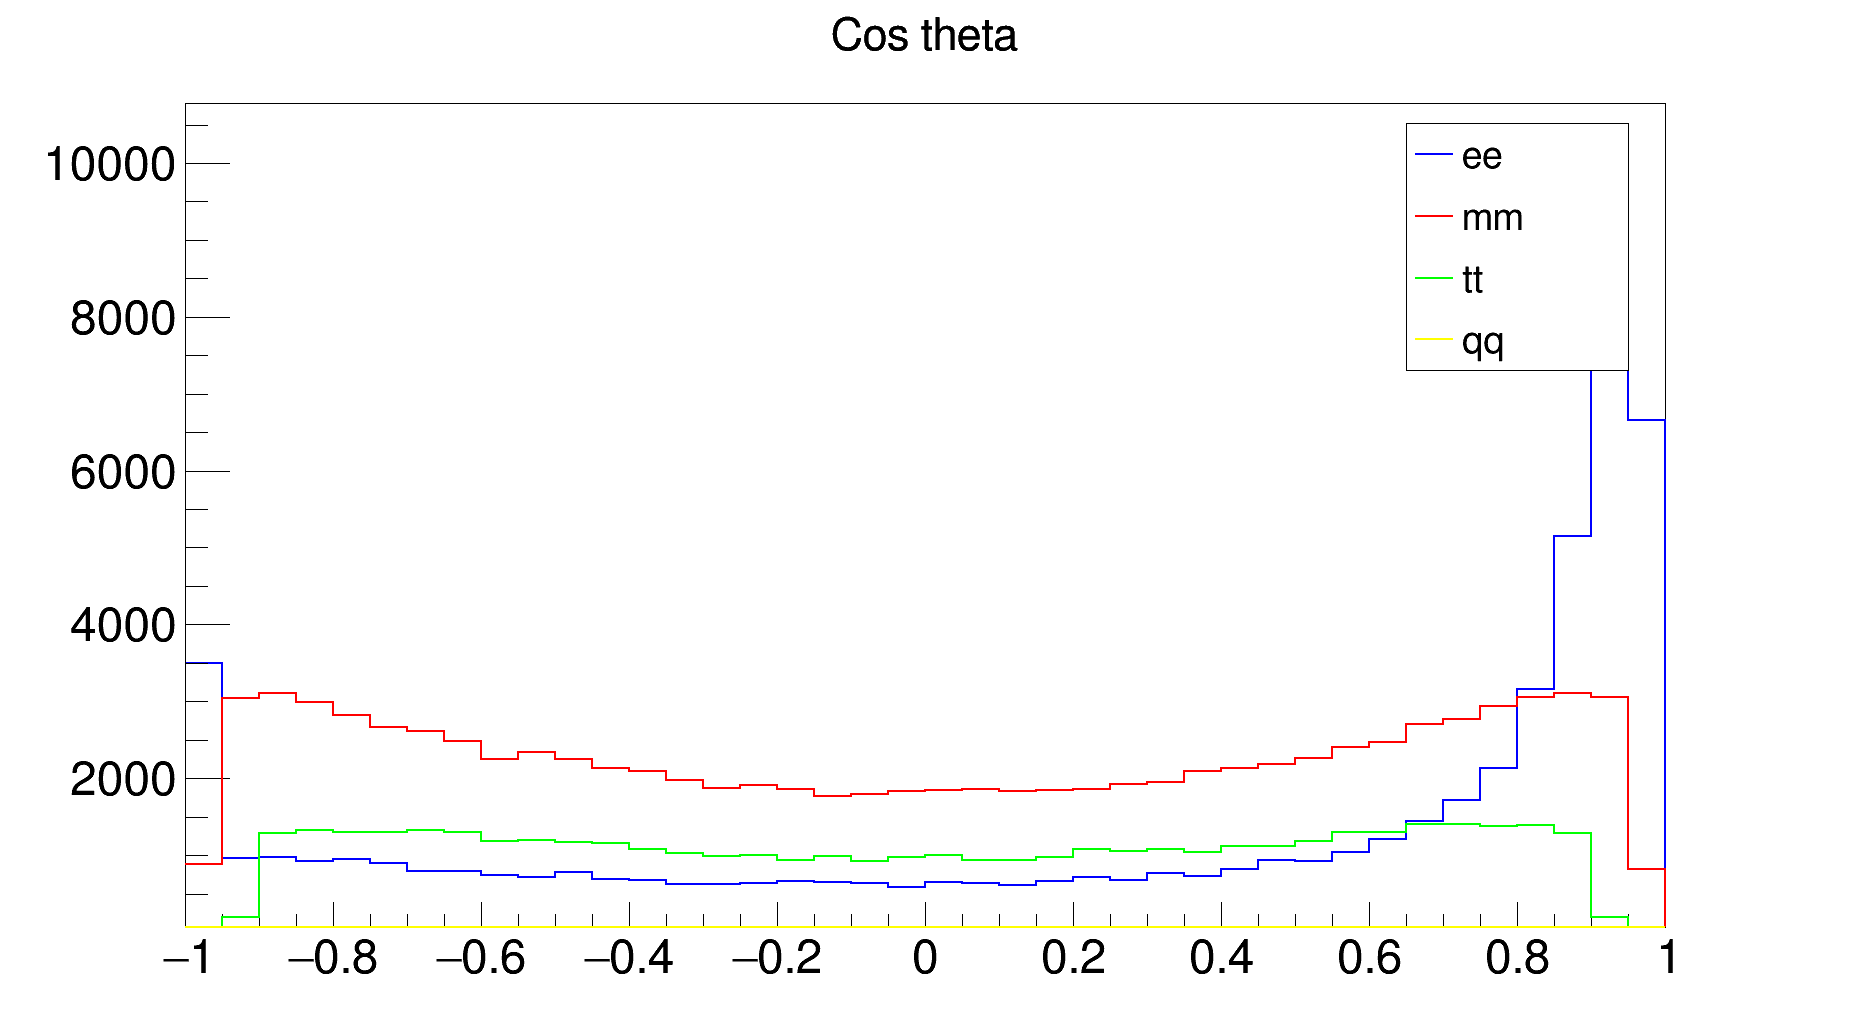
\includegraphics[width=1\linewidth]{../results/MC_results/nocut/cos_theta}
\caption[Cos\_theta in simulation data]{This figure shows the cosine of the angle between the beam and the direction of the created anti-lepton. Note the asymmetric peaks in the electron data, which will be discussed in the chapter on the separation of s- and t-channel.}
\label{fig:cos_theta}
\end{figure}

\subsubsection{Cuts in Cos\_theta}
As can be seen in figure \ref{fig:cos_theta}, the quark events are not assigned values of Cos\_theta within its natural boundaries from -1 to 1. This is due to the fact that they cause scattering jets, meaning that a well defined direction cannot be assigned. Leptonic events can also cause the creation of more than two particles. Furthermore, as there is no detection capacity in beam direction as well as for a very shallow angles, some regular events are also not assigned an angle. As a consequence, such events are listed with a Cos\_theta of $999.0$.\\
Since the electron data is later divided into s- and t-channel events, for which the Cos\_theta distribution is needed, it has to be ensured that the data is indeed valid. As there is no detection capacity for shallow angles to the beam direction, such events are cut off:

\begin{itemize}
	\item{\makebox[2.5cm][l]{\textbf{Electron cut}} $-0.9\le$ cos\_theta $\le0.9$}
\end{itemize}

\newpage
\begin{figure}[H]
\centering
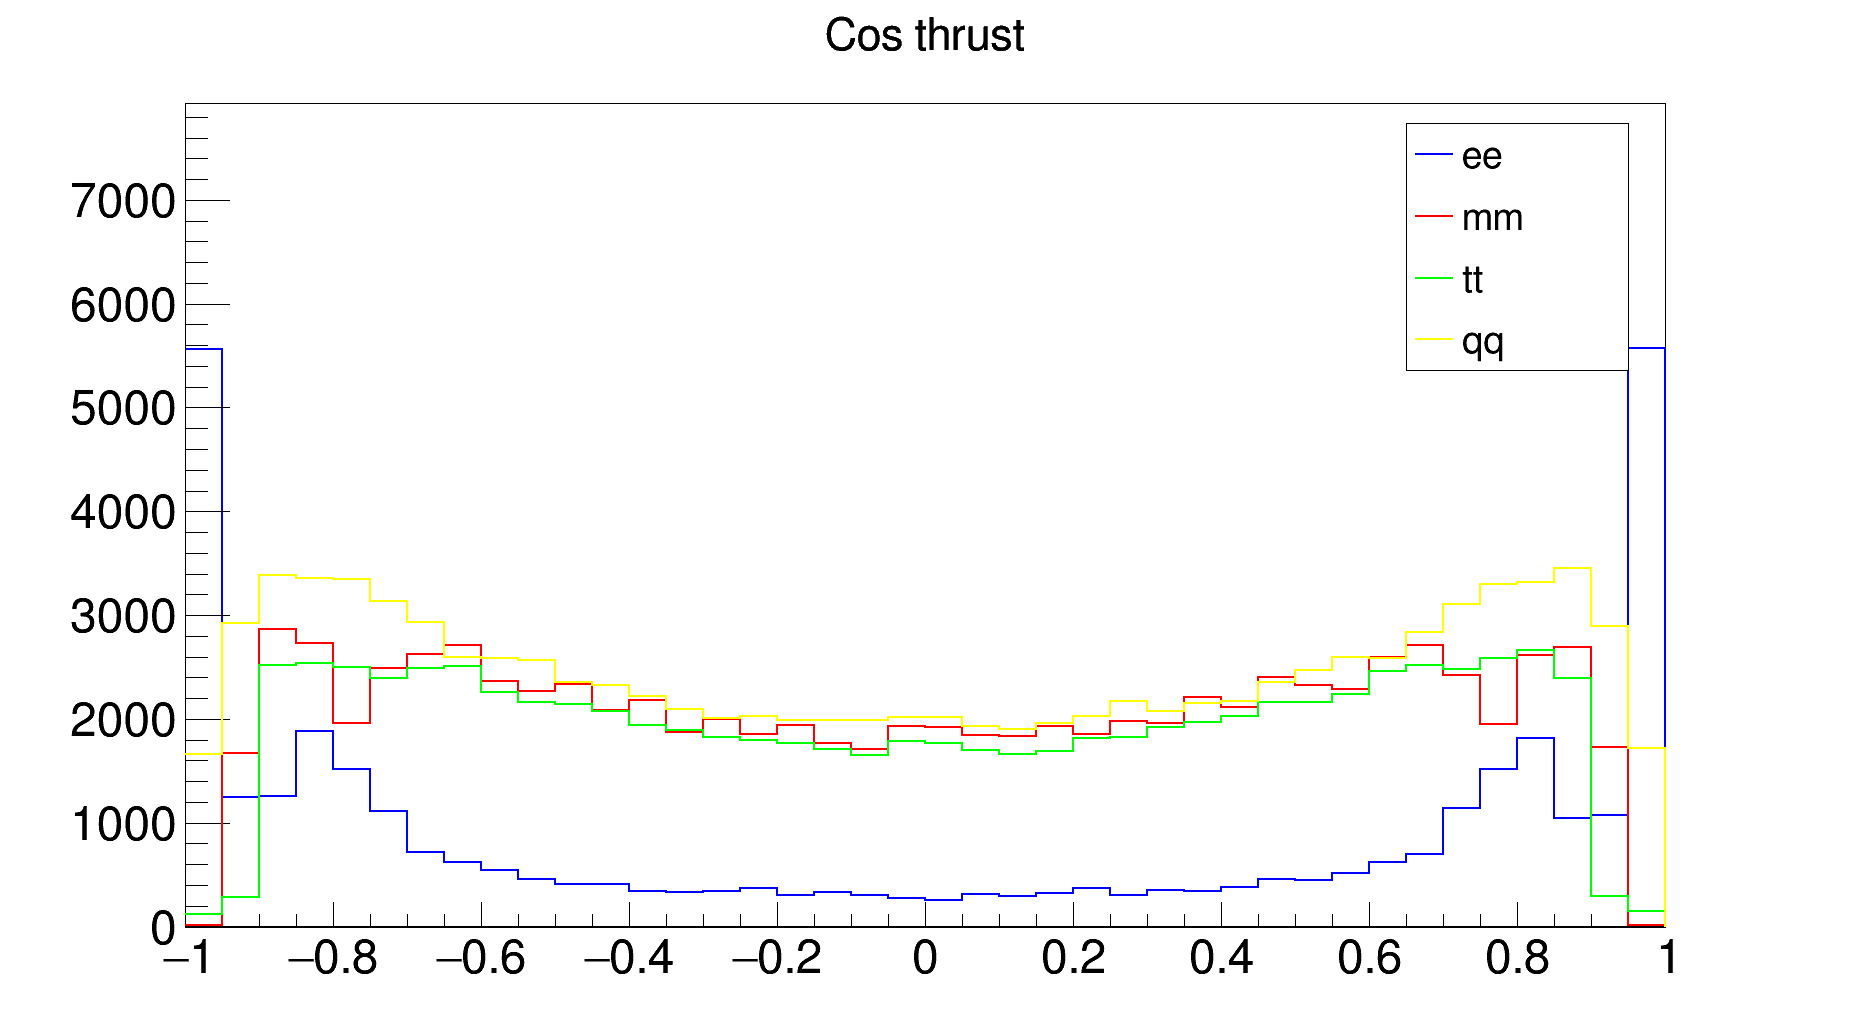
\includegraphics[width=1\linewidth]{../results/MC_results/nocut/cos_thru}
\caption[Cos\_thru in simulation data]{This figure shows the cosine of the angle between the beam and the thrust direction.}
\label{fig:cos_thru}
\end{figure}

\subsubsection{Cuts in Cos\_thrust}
Figure \ref{fig:cos_thru} suggests a cut to separate tauons from the rest of the particles, especially electrons, which often have have cos\_thrust $>0.9$ or cos\_thrust $<-0.9$.

\begin{itemize}
	\item{\makebox[2.5cm][l]{\textbf{Tauon cut}} $-0.9\le$ cos\_thrust $\le0.9$}
\end{itemize}

The final cuts thus are
\begin{table}[H]\centering
	\begin{tabular}{@{}llllllll@{}}
		\toprule
		&			&Ncharged	&Pcharged [GeV]	&E\_Ecal [GeV] &Cos\_theta				&Cos\_thrust\\ 
		\midrule
		&$e^+e^-$	&			&				&$\ge70$		&$\ge-0.9$ \& $\le0.9$	&\\
		&$\mu^+\mu^-$		&$=2$			&$\le60$		&$<50$			&						&\\
		&$\tau^+\tau^-$		&$<7$		&$>71$			&$<60$			&						&\\
		&$q\overline{q}$		&$\ge8$		&				&				&						&$\ge-0.9$ \& $\le0.9$	\\
		\bottomrule
	\end{tabular}
	\caption[Table of cuts]{Cuts applied to separate the datasets. An additional cut on Pcharged, which is not listed here, is discussed below.}
\end{table}
\newpage
\subsection{Two-photon events}
One possible source of background are two-photon events. Figure \ref{fig:twophotonfeynman} shows possible Feynman-graphs of such events. Two photons are created, without an intermediate Z$^0$. As such, these measurements need to be excluded using cuts.\\
In the event described by the Feynman graph on the right of figure \ref{fig:twophotonfeynman}, the incedent electron and proton scatter, but don't lose much energy in the process. They continue without diverging much from the beam direction. Naturally, there is no detecting capacity in beam direction, meaning these two particles are not registered. In the process of scattering, a fermion anti-fermion pair with low energy is created. They can be effectively cut by restricting Pcharged $> \unit{5}{GeV}$ without losing much in terms of efficiency.
As no charged particles are created in the event type described by the Feynman graph on the left of figure \ref{fig:twophotonfeynman}, the cut in Pcharged also effectively cuts against these kinds of events.
\begin{figure}[H]
\centering
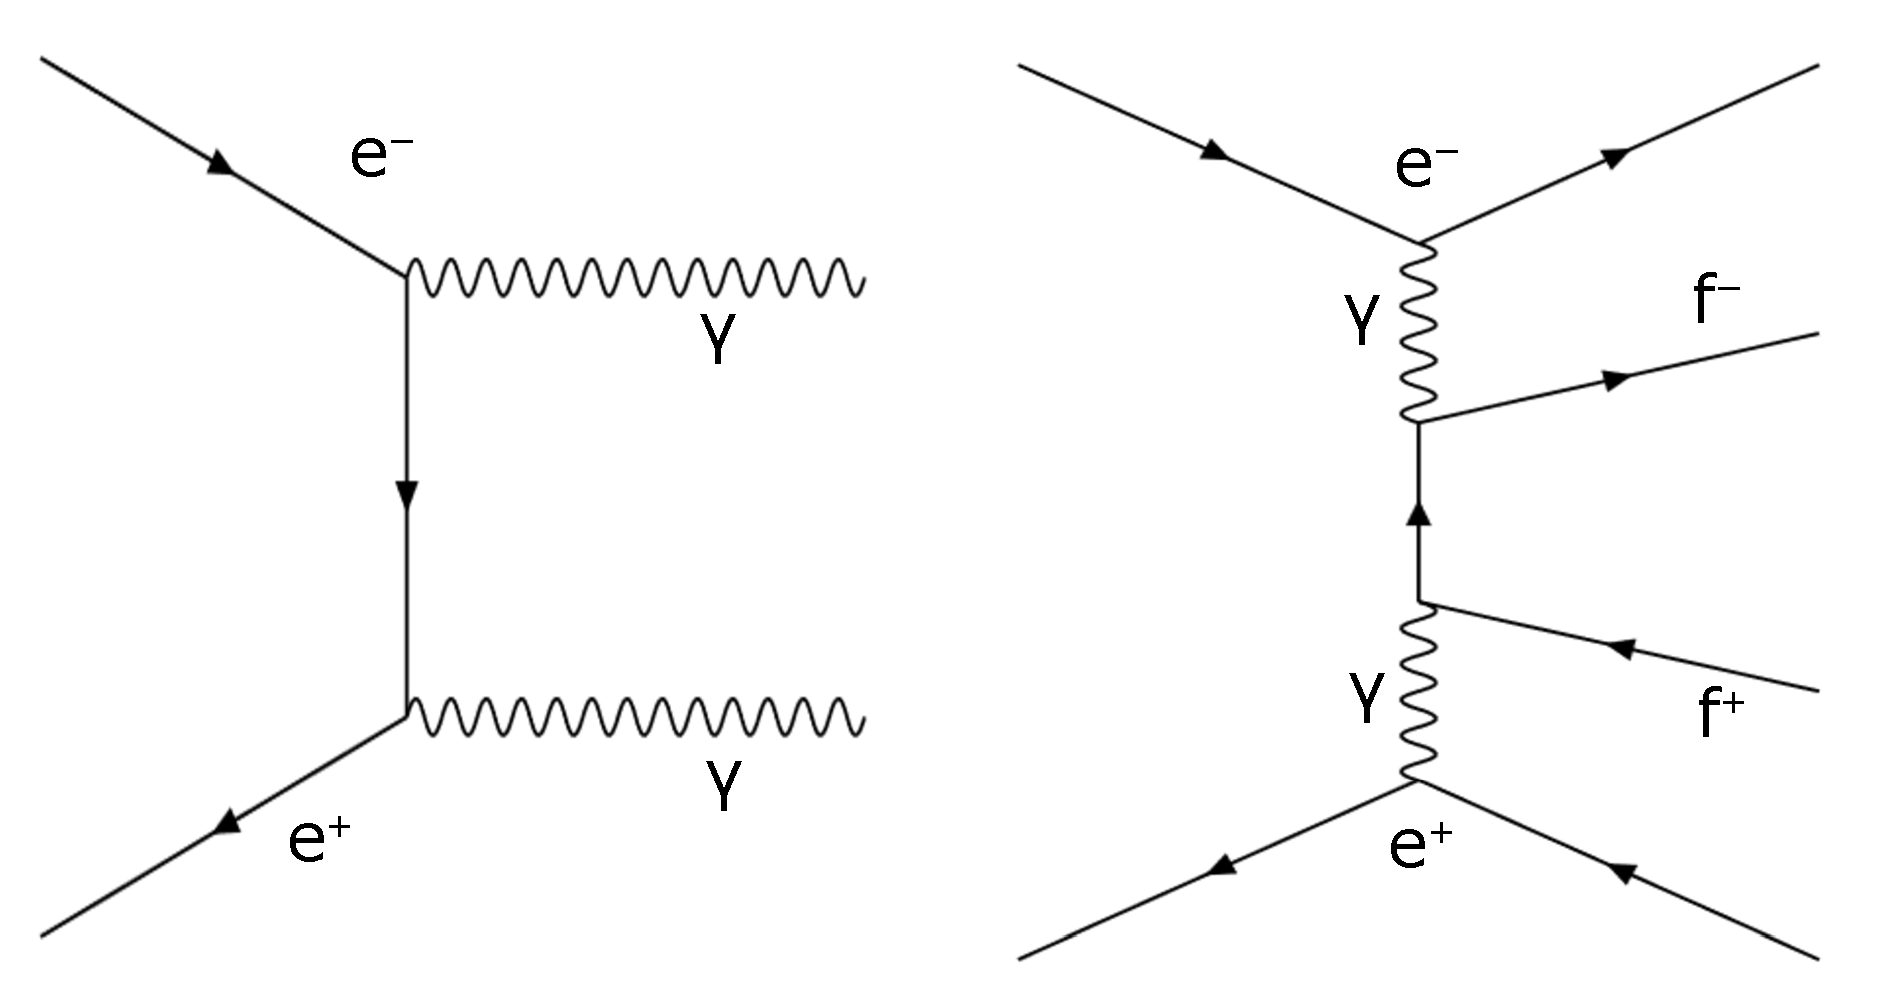
\includegraphics[width=1.0\linewidth]{graphics/twophotonfeynman_both.pdf}
\caption[Two-photon Feynman-graph]{Two examplary Feynman-graphs of two-photon events. A Z$^0$ is never created, which means that these event should not contribute to our measurement.}
\label{fig:twophotonfeynman}
\end{figure}

\subsection{Purity and the efficiency matrix}
These cuts are now applied to the simulated data, where the kind of event is known. This way, one can determine the efficiency and purity of the cuts and judge how well they work. 
The efficiency matrix is relatively easily calculated as
\begin{equation}
E_{ij}=\frac{n^{cut}_{ij}}{N_i}
\end{equation}
where the indexes $i$ and $j$ represent the kind of event. $n_{ij}^{cut}$ is thus the amount of events of type $i$ left over after applying the cut for type $j$ and $N_i$ is the overall number of events $i$ in the simulation data.
\begin{table}[H]\centering
	\begin{tabular}{@{}llllll@{}}
		\toprule
		&Events &$e^+e^-$&$\mu^+\mu^-$&$\tau^+\tau^-$&$q^+q^-$\\
		\midrule
		&Cut&&&&\\
		&$e^+e^-$&0.39078&0.00002&0.00422&0.00002\\
		&$\mu^+\mu^-$&0.00018&0.90171&0.00611&0.00001\\
		&$\tau^+\tau^-$&0.00039&0.00940&0.83413&0.00094\\
		&$q^+q^-$&0.00007&0.00001&0.00685&0.98437\\
	\end{tabular}
	\caption[Efficiency matrix]{Efficiency matrix of the applied cuts. The diagonal elements are the self efficiency.}
	\label{tb:efficiency}
\end{table}

As these values describe event counts, they should be distributed binomially. According to Paterno \cite{binpaper}, the binomial error of such values is commonly calculated as
\begin{equation}
s_{E_{ij}}=\sqrt{\frac{E_{ij}\cdot(1-E_{ij})}{N_i}}
\end{equation}
where $N_i$ is the number of simulated events of the appropriate kind. This yields the following matrix

\begin{table}[H]\centering
	\begin{tabular}{@{}llllll@{}}
		\toprule
		&Events &$e^+e^-$&$\mu^+\mu^-$&$\tau^+\tau^-$&$q^+q^-$\\
		\midrule
		&Cut&&&&\\
		&$e^+e^-$&0.001593&0.000015&0.000230&0.000014\\
		&$\mu^+\mu^-$&0.000044&0.000969&0.000277&0.000010\\
		&$\tau^+\tau^-$&0.000065&0.000314&0.001322&0.000098\\
		&$q^+q^-$&0.000028&0.000011&0.000293&0.000395\\
		\bottomrule
	\end{tabular}
	\caption[Efficiency error matrix]{Errors of the efficiency matrix elements calculated under the assumption of binomial distribution.}
	\label{tb:efficiencyerr}
\end{table}

To calculate the purity, it has to be taken into account that the different events do not occur with the same probability in nature but are roughly equally represented in the simulated data. This is expressed by the branching ratio
\begin{equation}
BR_i=\frac{\Gamma_i}{\sum_{i,j}\Gamma_{i}}
\end{equation}
where $\Gamma_i$ is the partial decay width corresponding to event $i$. The partial decay widths of leptons $\Gamma_l=\unit{83.8}{\mega\electronvolt}$ and of quarks $\Gamma_q=\unit{1732}{\mega\electronvolt}$ are given in \cite{staatsex} without error.
Using this, the purity can be calculated as
\begin{equation}
P_i=\frac{BR_i\cdot E_{ii}}{\sum_{j}BR_j\cdot E_{ij}}
\end{equation}
which yields the following results:

\begin{table}[H]\centering
	\begin{tabular}{@{}lll@{}}
		\toprule
		&Cut&Purity\\
		\midrule
		&$e^+e^-$&0.9882\\
		&$\mu^+\mu^-$&0.9928\\
		&$\tau^+\tau^-$&0.9661\\
		&$q\overline{q}$&0.9997\\
		\bottomrule
	\end{tabular}
	\caption[Purity of the cuts]{Purity of the cuts. All purities are above 95\%, indicating that the cuts work reasonably well.}
	\label{tb:purity}
\end{table}

\subsection{Calculation of the inverse efficiency matrix}
The efficiency matrix allows the calculation of the number of events after applying the cuts to a set of measurements where the kind of event is known:

\begin{equation}
\vec{C}=\boldsymbol{E}\cdot\vec{N}
\end{equation} 

where $\vec{N}$ is a vector whose components are the numbers of events of the four different kinds and $\vec{C}$ is a vector whose components are the number of events allocated to the four different cuts. 
In reality however, the kind of event is unknown and has to be determined by the cuts. Thus, the inverse of $\boldsymbol{E}$ can be used to calculate the number of actual events from the known number of events after the different cuts:
\begin{equation}
\vec{N}=\boldsymbol{E}^{-1}\cdot\vec{C}=:\boldsymbol{I}\cdot\vec{C}
\label{eq:numberevents}
\end{equation} 
The inverse matrix $\boldsymbol{I}$ is
\begin{table}[H]\centering
	\begin{tabular}{@{}llllll@{}}
		\toprule
		&Events &$e^+e^-$&$\mu^+\mu^-$&$\tau^+\tau^-$&$q^+q^-$\\
		\midrule
		&Cut&&&&\\
		&$e^+e^-$&2.55899&0.00007&-0.01294&-0.00004\\
		&$\mu^+\mu^-$&-0.00051&1.10909&-0.00812&-0.00000\\
		&$\tau^+\tau^-$&-0.00120&-0.01250&1.19896&-0.00115\\
		&$q^+q^-$&-0.00019&0.00008&-0.00835&1.01589\\
		\bottomrule
	\end{tabular}
	\caption[Inverse efficiency matrix]{The inverse of the efficiency matrix displayed in table \ref{tb:efficiency}.}
	\label{tb:invefficiency}
\end{table}

To calculate the error of the inverse matrix, a method called \emph{toy experiments} has to be used. A normal-distribution random variable $G=\mathcal{N}(0,1)$ is multiplied by the error of an element of the efficiency matrix and then added to said element.
\begin{equation}
E^{k}_{ij}=E_{ij}+G^k\cdot s_{E_{ij}}
\end{equation}
This is done $N=100000$ times, resulting in 100000 randomly varied efficiency matrix, which are then inverted. The standard deviation of the thus calculated elements $I^k_{ij}$ of the inverse matrix is used as the error for the inverse matrix elements $I_{ij}$: 
\begin{equation}
s_{I_{ij}}=\sqrt{\frac{1}{N-1}\sum_{k=1}^{N}\left(I^k_{ij}-I_{ij}\right)^2}
\end{equation}
The resulting matrix is displayed in table \ref{tb:invefficiencyerror}
\begin{table}[H]\centering
	\begin{tabular}{@{}llllll@{}}
		\toprule
		&Events &$e^+e^-$&$\mu^+\mu^-$&$\tau^+\tau^-$&$q^+q^-$\\
		\midrule
		&Cut&&&&\\
		&$e^+e^-$&0.010372&0.000043&0.000703&0.000037\\
		&$\mu^+\mu^-$&0.000123&0.001187&0.000366&0.000011\\
		&$\tau^+\tau^-$&0.000196&0.000416&0.001870&0.000119\\
		&$q^+q^-$&0.000074&0.000013&0.000353&0.000403\\
		\bottomrule
	\end{tabular}
	\caption[Inverse efficiency error matrix]{Errors of the inverse efficiency matrix (table \ref{tb:invefficiency}) calculated using the \emph{toy experiments} method.}
	\label{tb:invefficiencyerror}
\end{table}

\subsection{Separation of s- and t-channel}
The electron data still includes the scattering events (t-channel), where no real $Z^0$ is created. The results from these measurements thus give no information about the properties of the $Z^0$ boson and need to be excluded from the results. In section \ref{sec:ee interaction}, it was explained that these two kinda of events show different angular distributions. A linear combination of said distributions, $\sigma_s$ and $\sigma_t$ (equation \ref{eq:principles:s-t-channel}),
\begin{equation}
N(x)=A_s\cdot(1-x^2)+A_t\cdot(1-x)^{-2}
\end{equation}
where $A_s$ and $A_t$ are fit parameters and $x=$cos\_theta is the variable, was fitted to the cos\_theta-channel data of the events classified by the cuts as electron events. The result can be seen in figure \ref{fig:stchannelseparation}.
\begin{figure}
\centering
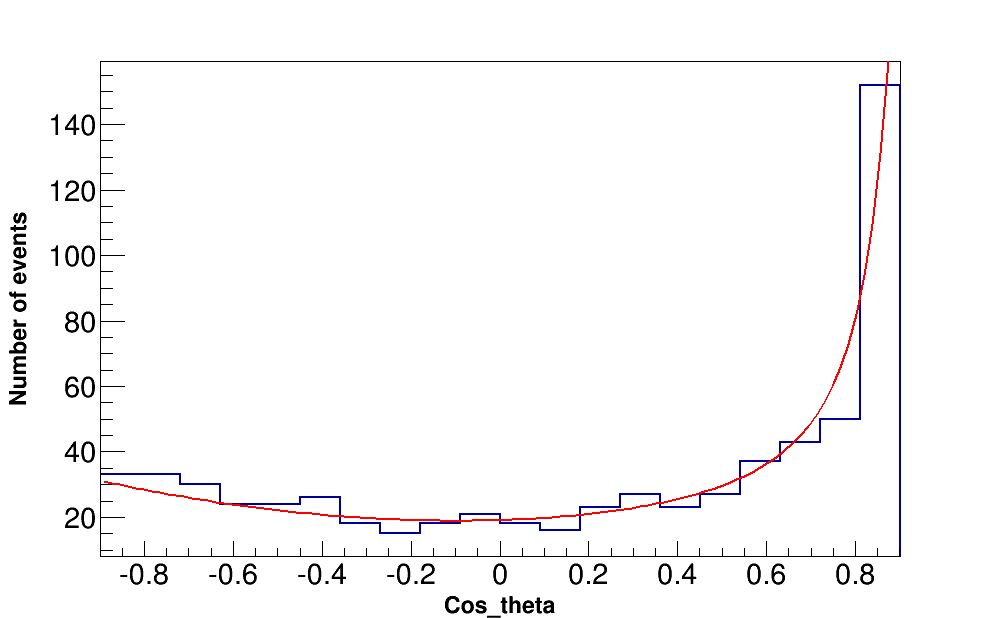
\includegraphics[width=1.0\linewidth]{../results/data_results/cosp_fits/stchannelexample46.png}
\caption[s-t-channel separation $\sqrt{s}\approx\unit{92}{GeV}$ GeV]{S-t channel separation for $\sqrt{s}\approx\unit{92}{GeV}$. The electron cut limits cos\_theta to the range $-0.9\le$cos\_theta$\le0.9$.}
\label{fig:stchannelseparation}
\end{figure}
The number of events in the s-channel $N_s$ and t-channel $N_t$ can then be calculated by integrating the summands respectively
\begin{equation}
N_s=s\cdot\int_{-0.9}^{0.9}1+x^2dx=:s\cdot I_s,\qquad N_t=t\cdot\int_{-0.9}^{0.9}(1-x)^{-2}dx=:t\cdot I_t
\end{equation}
The integrals are mere constants,$I_s\approx2.3$ and $I_t\approx9.5$, thus making the error calculations simpler as they might seem on first glance. The following quotient can later be used to correct the number of $e^+e^-$-events after the cuts
\begin{equation}
c_{st}=\frac{N_s}{N_s+N_t},\qquad s_{c_{st}}=\sqrt{\left(\frac{I_s\cdot N_t}{(N_s+N_t)^2}\cdot s_s\right)^2+\left(\frac{I_t\cdot N_s}{(N_s+N_t)^2}\cdot s_t\right)^2}
\end{equation}

\subsection{Cross sections and the mass of Z$^0$}
With the data cleared of underground effects, the cross sections can be calculated. The number of events after the respective cuts $\vec{C}$ are Poisson-distributed, thus
\begin{equation}
s_{C_i}=\sqrt{C_i}
\end{equation}
With equation \ref{eq:numberevents}, the error on the events $\vec{N}$ that presumably occurred can be calculated as
\begin{equation}
s_{N_i}=\sqrt{\sum_{i,j}\left((C_j\cdot s_{I_{ij}})^2+(I_{ij}\cdot s_{M_j})^2\right)}
\end{equation}
For electron-positron events, the s-t-channel separation has to be implemented:
\begin{equation}
N'_{e^+e^-}=c_{st}\cdot N_{e^+e^-}, \qquad s_{N'_{e^+e^-}}=\sqrt{(c_{st}\cdot s_{N_{e^+e^-}})^2+(N_{e^+e^-}\cdot s_{c_{st}})^2}
\end{equation}
In order to calculate the cross sections, the radiation corrections and the luminosity of the accelerator are needed. Both were provided and are listed in the following table

\begin{table}[H]\centering
	\begin{tabular}{@{}llllllll@{}}
		\toprule
		  &$\sqrt{s}$ [GeV]	&L [\nicefrac{1}{nb}]	&$s_L^{stat}$[\nicefrac{1}{nb}]	&$s_L^{sys}$[\nicefrac{1}{nb}]	&$s_L^{total}$[\nicefrac{1}{nb}]&$c_{beam,l^+l^-}$ [nb]&$c_{beam,q\overline{q}}$ [nb]\\
		  \midrule
		  &88.48	&675.9	&3.5	&4.5	&5.7	&0.09	&2.0\\  
		  &89.47	&543.6	&3.2	&3.6	&4.8	&0.20	&4.3\\  
		  &90.23	&419.8	&2.8	&2.8	&4.0	&0.36	&7.7\\  
		  &91.23	&3122.2	&7.8	&20.9	&22.3	&0.52	&10.8\\  
		  &91.97	&639.8	&3.6	&4.2	&5.6	&0.22	&4.7\\  
		  &92.97	&479.2	&3.1	&3.2	&4.5	&-0.01	&0.2\\  
		  &93.72	&766.8	&4.0	&5.1	&6.5	&-0.08	&-1.6\\
		\bottomrule
	\end{tabular}
	\caption[Table of luminosities]{The luminosities L and radiation corrections $c_{beam}$ for the different mean energies $\sqrt{s}$. The radiation corrections where found in \cite{anleitung}, where no error was given.}
	\label{tb:luminosity}
\end{table}

The cross section and their error can then be calculated as
\begin{equation}
\sigma_i=\frac{N_i}{L}+c_{beam,i}, \qquad s_{\sigma_i}=\sqrt{(\frac{s_{N_i}}{L})^2+(\frac{N_i\cdot s_L^{total}}{L^2})^2}
\end{equation}

Figure \ref{fig:WQmm} shows the result of the calculations for the muon cut (for the other graphs, see appendix). The Breit-Wigner function from equation \ref{eq:principles:breitwigner} was changed to be
\begin{equation}
\sigma_f(s) = \frac{12\pi}{M_Z^2} \frac{s\Gamma_f^2}{(s-M_Z^2)^2+s^2\Gamma_Z^2/M_Z^2}
\end{equation}
where, instead of $\Gamma_e\Gamma_f$, $\Gamma_f^2$ was used for all fits, reducing the number of fit parameters. For the leptons, this means assuming lepton universality. For the hadrons, this makes an additional calculation, which will be discussed in the next section. This function was used for all of the following fits.

\begin{figure}
\centering
\includegraphics[width=1.0\linewidth]{../results/data_results/wqs/WQmm}
\caption[Cross sections for muon cut]{Cross sections of the different $\sqrt{s}$ in the muon cut. The graphs for the other cuts can be found in the appendix.}
\label{fig:WQmm}
\end{figure}

The fits yielded the following values for the mass of the Z$^0$-boson
\begin{table}[H]\centering
	\begin{tabular}{@{}llll@{}}
		\toprule
		&Event type&$M_{Z^0}$ [GeV]&$s_{M_{Z^0}}$ [GeV]\\
		\midrule
		&$e^+e^-$&91.11&0.06\\
		&$\mu^+\mu^-$&91.20&0.03\\
		&$\tau^+\tau^-$&91.18&0.04\\
		&$q\overline{q}$&91.189&0.009\\
		\midrule
		&Weighted mean&91.188&0.008\\
		&Literature value&91.187&\\
		\bottomrule
	\end{tabular}
	\caption[Breit-Wigner fit results: $M_{Z^0}$]{The mass of Z$^0$ as it was calculated from the fits for the different cuts as well as their weighted mean. The literature value was found in \cite{muenchen} (no error listed).}
	\label{tb:Z0massfitresults}
\end{table}

The weighted mean is in very good agreement with the literature value, enclosing it in its relatively small (<0.01\%) $1\sigma$ interval.

\subsection{Decay widths and the neutrino generations}
The Breit-Wigner fits also included the decay widths as fit parameters. The results are listed in table \ref{tb:decaywidthfitresults}.  

\begin{table}[h]\centering
	\begin{tabular}{@{}llllllll@{}}
		\toprule
		&Event $i$&$\Gamma_{Z}$ [GeV]&$s_{\Gamma_{Z}}$ [GeV]&$\Gamma_i$ [MeV]&$s_{\Gamma_i}$ [MeV]&$\Gamma^{lit}_i$ [MeV]&$\Gamma^{calc}_i$ [MeV]\\
		\midrule
		&$e^+e^-$&2.28&0.11&94&4&83.8&83.4\\
		&$\mu^+\mu^-$&2.52&0.06&82.9&1.7&83.8&83.4\\
		&$\tau^+\tau^-$&2.48&0.07&76.9&1.9&83.8&83.4\\
		&$q\overline{q}$&2.526&0.019&1777&41&1732&1742\\
		\bottomrule
	\end{tabular}
	\caption[Breit-Wigner fit results: Decay widths ]{The decay widths resulting from the Breit-Wigner fits and their literature value (from \cite{staatsex}, nor error given) for comparison. The values that were theoretically calculated by the authors during the preparation for the experiment are listed in the last column.}
	\label{tb:decaywidthfitresults}
\end{table}

The partial decay width $\Gamma_q$ of the quark events was calculated from the fit parameter $\Gamma_f^q$ as
\begin{equation}
\Gamma_q=\frac{(\Gamma_{f}^q)^2}{\Gamma_e},\qquad
s_{\Gamma_q}=\sqrt{\left(\frac{2\Gamma_f^q}{\Gamma_e}\cdot s_{\Gamma_f^q}\right)^2+\left(\frac{(\Gamma_f^q)^2}{\Gamma_e^2}\cdot s_{\Gamma_e}\right)^2}
\end{equation}
where the results from the muon fits were used for the partial decay width of the electron $\Gamma_e$. This can be done since we have already assumed lepton universality and is reasonable, because the electron results include the s-t-channel separation, which, as discussed, is a significant source of error. Furthermore, the purity (table \ref{tb:purity}), was the highest for muon cuts, while the efficiency was still the best for among the lepton cuts.\\
The tauon events are a less reliable source due to their comparatively complex signature (see figure \ref{fig:tauonopal}). As a result, the simulated tauon data showed significant overlaps with the other data sets in all analysis channels, thus making it difficult to define efficient cuts with high purity. 
Incidentally, the muon events are also the only lepton event that includes the literature and theoretical values in their $1\sigma$ interval. The results for the electron events is higher than expected and includes said values only in its $3\sigma$ interval. This is likely due to the s-t-channel separation. If not all Bhabha scattering events are excluded, the cross section increases and with it does the decay width resulting from the fits. More data could improve the fit that was done to the cos\_theta distribution of the electron cuts. \\

To calculate the amount of neutrino generations $n_{\nu-gen}$, on first has to calculate the blind decay width
\begin{equation}
	\Gamma_{blind}=\Gamma_{Z}^{ave}-3\cdot\Gamma_e-\Gamma_{q\overline{q}}=\unit{(0.49\pm0.04)}{GeV}
\end{equation}
where $\Gamma_{Z}^{ave}=\unit{(2.516\pm0.017)}{GeV}$ is the weighted average of the four calculated $\Gamma_{Z}$. Again assuming lepton universality, the muon result was used for $\Gamma_e$.
The blind decay width is then divided by the theoretically calculated decay width $\Gamma_{\nu}^{calc}=\unit{0.1676}{GeV}$ (see table \ref{tb:appendix:decay widths}) of a single neutrino generation.
\begin{equation}
	n_{\nu-gen}=\frac{\Gamma_{blind}}{\Gamma_{\nu}^{calc}}=(2.9\pm0.5)
\end{equation}
While the relative error,being roughly 17\%, is large, the only integer that the $1\sigma$ interval encloses is 3. Since the $2\sigma$ interval additionally includes 2 and the $3\sigma$ interval encloses 4, the results suggest that there are 3 neutrino generations, but do not satisfactory rule out the possibility that there are 2 or 4 neutrino generations.


\subsection{Forward-backward asymmetry}
The forward ($0<$ cos\_theta $<1$) and backward ($-1<$ cos\_theta $<0$) events were counted for the second, forth and sixth center-of-mass energies, $\sqrt{s}\approx89.5\text{, }91.23$ and $\unit{93.0}{GeV}$. This represents the integrals in equation \ref{eq:priciples:fbintegral}, as the cross sections are proportional to the number of events. The asymmetry can then be calculated as
\begin{equation}
A_{fb}=\frac{N_f-N_b}{N_f+N_b},\qquad s_{A_{fb}}=2\sqrt{\frac{N_f^2s_{N_b}^2+N_b^2s_{N_f}^2}{(N_f+N_b)^4}}=2\sqrt{\frac{N_fN_b}{(N_f+N_b)^3}}
\end{equation}
where $N_f$ and $N_b$ are the event counts, $s_{N_f}=\sqrt{N_f}$ and $s_{N_b}=\sqrt{N_b}$ are their binomial errors, thus justifying the simplification in above equation. 
Equation \ref{eq:principles:asymmetry weinberg angle} now allows the calculation of the Weinberg angle. For that it has to be solved for the angle
\begin{equation}
\theta_w=\arcsin(\sqrt{\frac{1-\sqrt{A_{fb}/3}}{4}}),\qquad s_{\theta_w}=\frac{1}{4}\sqrt{-\frac{s_{A_{fb}}^2}{A_{fb}(\sqrt{12A_{fb}}+A_{fb}-9)}}
\end{equation}
Table \ref{tb:weinbergangle} shows the results of this calculation. Inserting the value $\theta_w=28.7$ ° \cite{Grif} in equation \ref{eq:principles:asymmetry weinberg angle} yields an expected asymmetry of $A_{bf}^{lit}\approx0.018$.\\
\begin{table}[h]\centering
	\begin{tabular}{@{}llllllll@{}}
		\toprule
		&$\sqrt{s}$ [GeV]&$N_f$&$N_b$&$A_{fb}$&$s_{A_{fb}}$&$\theta_w$ [°]&$s_{\theta_w}$ [°]\\
		\midrule
		&89.5&117&112&0.02&0.07&28.6&2.2\\
		&91.23&1845&1881&-0.010&0.016&&\\
		&93.0&153&99&0.21&0.06&25.3&0.7\\
		\bottomrule
	\end{tabular}
	\caption[A\_{fb} and the Weinberg angle]{The Weinberg angle for calculated for three different center-of-mass energies. The Weinberg angle can be found in \cite{muenchen} as $\theta_w^{lit}=28.7426$°. Calculations for $\sqrt{s}\approx\unit{91.23}{GeV}$ yielded complex angles.}
	\label{tb:weinbergangle}
\end{table}
As the asymmetry is negative for $\sqrt{s}\approx\unit{91.23}{GeV}$, the calculated Weinberg angle is complex. The $1\sigma$ interval around the asymmetry includes positive values and the $2\sigma$ interval includes the expected value for the asymmetry. In fact, all values for the asymmetry include the expected value, but their errors margins, in particular that for $\sqrt{s}\approx\unit{89.5}{GeV}$ being  $>300\%$, are very wide. This stems from the low number of counts and the fact that a difference of two values with a large relative error is calculated. More data would greatly increase the accuracy and allow for more reliable results for the asymmetry.\\
According to \cite{muenchen}, the Weinberg angle itself can also be calculated as from the mass of the $Z^0$-boson and some constants. 
\begin{equation}
\begin{aligned}
\theta_w&=\arcsin\left(\sqrt{\frac{1}{2}-\sqrt{\frac{1}{4}-\frac{\pi\cdot\alpha(M_Z^2)}{\sqrt{2}\cdot G_F\cdot M_Z^2}}}\right)\\
s_{\theta_w}&=\sqrt{\frac{\pi}{4\sqrt{2}}}\cdot\sqrt{\frac{s_{M_Z}^2\cdot\alpha(M_Z^2)}{M_Z^2\cdot(G_FM_Z-2\sqrt{2}\pi\alpha(M_Z^2))}}
\end{aligned}
\end{equation}
Converted to degrees, the results it $\theta_w=(28.746\pm0.004)$°, which encloses the literature value $\theta_w^{lit}=28.7426$° \cite{muenchen} in its $1\sigma$ interval.


